\section{Overview}
\label{sec:overview}
\begin{figure*}[t]
  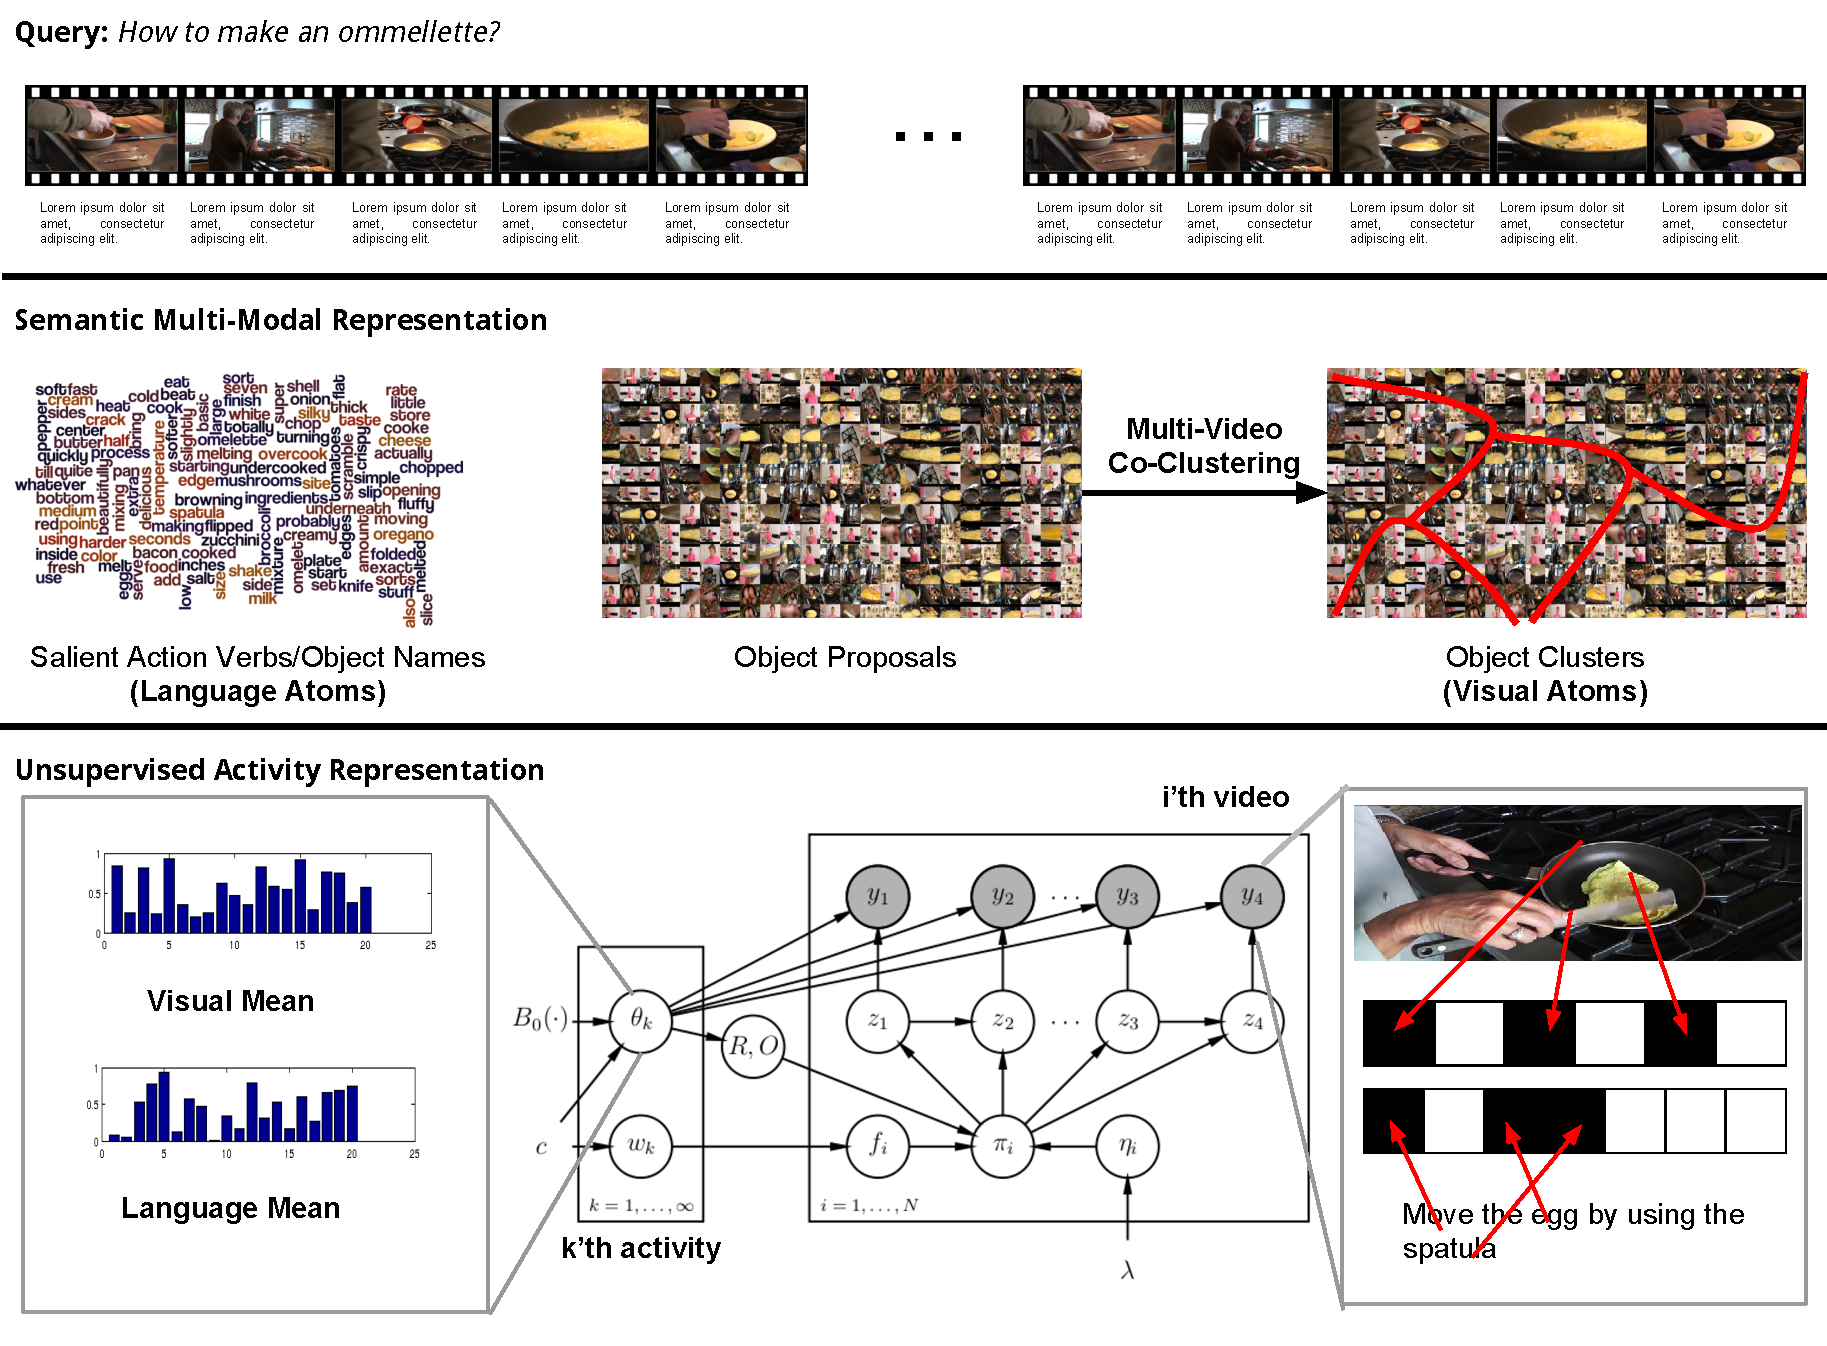
\includegraphics[width=\textwidth]{algor}
  \caption{Components of our recipe understanding method. \textbf{Query:} We query the YouTube for top 100 \emph{How To} videos and filter the outliers; \textbf{Framewise Representation:} We automatically extract object clusters and salient word in order to find multi-modal representation of each frame. \textbf{Unsupervised Activity Detection:} We jointly cluster videos in order to learn activities/steps related to the recipe.}
\label{fig:overview}
\end{figure*}

In this section, we explain the high-level components of our method which we visualize in Figure~\ref{fig:overview}. Our proposed method consists of three major components; \textbf{(1) Online query and filtering:} Our system starts with querying the YouTube with an \emph{How to} question, and records the top 100 resulting videos. In order to detect the similarity of the videos quickly, we also process the text descriptions and eliminate outliers. \textbf{(2) Frame-wise multi-modal representation:} In order to semantically represent the spatio-temporal information in the videos, we process both the visual and language content of each video. We extract the region proposals and jointly cluster them to detect semantic visual objects. We also detect the salient words of the subtitles. Finally, we epresent the each frame in terms of the resulting objects and the salient words. \textbf{(3) Unsupervised joint clustering:} After describing the each frame by using both language and visual cues, we apply a non-parametric Bayesian method in order to find the temporally consistent clusters (collection of video clips) occurring over multiple videos. We expect these clusters to correspond to the actions which construct the high level activities. Moreover, our empirical results suggest that the resulting clusters significantly correlates with the fine-grained activities.

We now explain the details of the each sub-system in the following sections.
